\section{DMA (Direct Memory Access)}\label{par:DMA}

Il \textbf{DMA} è un dispositivo che permette di sollevare il processore dall'onere di trasferire i dati tra varie periferiche. Questo significa che i dispositivi possono comunicare direttamente con la memoria senza passare per la CPU. In particolare, il DMA permette di gestire il trasferimento dati tra:
\begin{itemize}
    \item \textbf{Memoria $\leftrightarrow$ Periferica};
    \item \textbf{Periferica $\leftrightarrow$ Memoria};
    \item \textbf{Memoria $\leftrightarrow$ Memoria}.
\end{itemize}

Il suo principio di funzionamento è semplice, ed è schematizzabile tramite tre registri principali:
\begin{itemize}
    \item \textbf{Registro Indirizzo}: indica l'indirizzo da cui prelevare il dato;
    \item \textbf{Registro Conteggio}: indica il conteggio del numero di dati trasferiti e permette di capire quando interrompere il trasferimento;
    \item \textbf{Registro Identificativo}: tramite tale registro si identifica:
    \begin{itemize}
        \item o il dispositivo da considerare per il trasferimento;
        \item o l'area di memoria da considerare per il trasferimento.
    \end{itemize}  
\end{itemize}

La reale architettura del DMA è però più complessa. La maggior complessità dell'architettura proviene da varie problematiche che si possono riscontrare durante il funzionamento, come, ad esempio, l'accesso al BUS dati in maniera concorrente al processore. \uppercase{È} pertanto necessario che il DMA non sia collegato al processore solo tramite il bus dati, ma anche tramite vari segnali di controllo, che permettono al processore e al DMA di potersi coordinare.

Il dispositivo di riferimento nelle esercitazioni del corso è l'\textbf{Intel 8237}, che per la sua architettura dispone di 4 canali per il collegamento con 4 dispositivi diversi. Nella versione simulata in ASIM, tale componente è composto di soli 2 canali.

Scendendo più nei dettagli, il dispositivo reale è in grado di sostenere 4 modalità di funzionamento differenti:
\begin{itemize}
    \item \textbf{Single}: si trasferisce una \textit{word} alla volta; dopo aver trasferito una word, il DMA restituisce il BUS al processore almeno per un ciclo;
    \item \textbf{Block}: si trasferisce un intero \textit{blocco} non appena il DMA acquisisce il BUS. Alla fine del trasferimento viene inoltrata un'interruzione al processore che segnala la disponibilità del BUS;
    \item \textbf{On Demand}: simile alla modalità Block, con la differenza che il trasferimento può essere interrotto dal processore e poi ripreso, grazie ai registri contatore, dall'esatto punto in cui era stato interrotto;
    \item \textbf{Cascade}: modalità di funzionamento che permette di collegare più DMA in cascata per gestire più di 4 canali.
\end{itemize}

Il DMA acquisisce il controllo del bus attraverso il seguente processo (fare riferimento alla figura \ref{img:architettura-dma}):
\begin{itemize}
    \item IL DMA richiede il possesso del bus al processore tramite il segnale BR Bus Request;
    \item Il processore fornisce il consenso alla richiesta di utilizzo del bus tramite il segnale BG Bus Grant;
    \item Il dispositivo che ha richiesto il bus fornisce l'ack al processore mediante il segnale BGACK, e il processore viene scollegato elettricamente dal BUS indirizzi.
\end{itemize}
Il DMA si interfaccia con le periferiche mediante i segnali DREQ e DACK: DREQ è una richiesta da parte della periferica per il DMA di un trasferimento dati, mentre DACK è la comunicazione da parte del DMA che un dispositivo è stato selezionato per un trasferimento, ed è propagato una volta che il DAC ha acquisito l'accesso al bus indirizzi.


Oltre al minor numero di canali, il componente simulato in ASIM non supporta tutte le modalità sopra citate: le modalità utilizzabili in ASIM sono infatti \textbf{Single} e \textbf{Block}.

Guardando la figura~\ref{img:DMA}, abbiamo il modello architetturale del componente realizzato in ASIM, in cui i registri posti sulla sinistra sono di comunicazione con il processore, mentre i segnali sulla destra servono per l'interfacciamento con le periferiche collegate ai canali.

Per la comunicazione con il processore, i segnali rappresentati hanno il seguente significato:
\begin{itemize}
    \item \textbf{D0-D7}: collegamento al BUS dati da e verso il componente;
    \item $\overline{\mathbf{CS}}$: segnale binario di selezione del dispositivo;
    \item \textbf{A0-A3}: attenzione! Non tutti i segnali $A_i$, ma solo i 4 meno significativi, vengono utilizzati per la selezione dello specifico registro interno;
    \item $\overline{\mathbf{IOR}}$ e $\overline{\mathbf{IOW}}$: segnali di gestione della lettura e della scrittura sul componente e sulle periferiche;
    \item $\overline{\mathbf{MEMR}}$ e $\overline{\mathbf{MEMW}}$: segnali di gestione della lettura e della scrittura sui dispositivi di memoria;
    \item \textbf{CLK e Reset}: classici segnali di clock (tempificazione) e reset dei registri del dispositivo;
    \item \textbf{HRQ}: segnale di richiesta del controllo del sistema BUS, solitamente collegato all'ingresso HOLD della CPU;
    \item \textbf{HLDA}: segnale proveniente dalla CPU che segnala l'acquisizione del BUS da parte del processore;
    \item $\overline{\mathbf{EOP}}$: linea di interruzione \textit{bidirezionale} che si collega al processore per segnalare il completamento del trasferimento.
\end{itemize}

Dati i due differenti canali, si avranno due periferiche collegate allo stesso dispositivo DMA. La comunicazione può essere effettuata da una sola periferica per volta. Tale decisione è presa secondo un ordine di priorità, per cui il dispositivo collegato ai terminali 0 ha priorità maggiore rispetto a quello collegato ai terminali 1. I segnali che gestiscono le periferiche sono:

\begin{itemize}
    \item \textbf{DREQ0 e DREQ1}: segnali usati dalle periferiche per richiedere l'accesso al BUS tramite cicli DMA;
    \item \textbf{DACK0 e DACK1}: segnali con cui il DMA comunica alla periferica la disponibilità a soddisfare la richiesta.
\end{itemize}

\begin{figure}[ht]
    \centering
    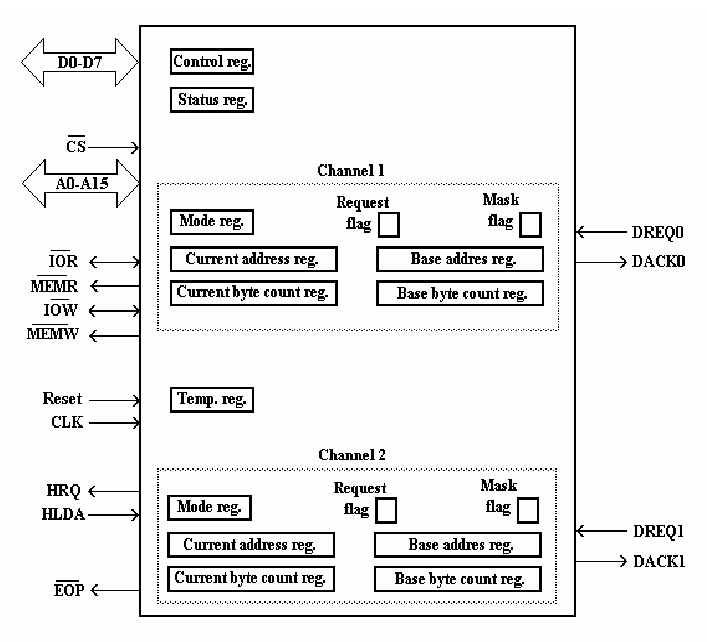
\includegraphics[width=.7\textwidth]{img/DMA.png}
    \caption{Modello di programmazione DMA a 2 canali}
    \label{img:DMA}
\end{figure}

Consideriamo il canale 0 del DMA, ed analizziamo il modello di programmazione.
Il registro CADDR0 (Current Adress) contiene l'indirizzo della locazione di memoria interessata dal trasferimento, ed è accessibile in lettura e scrittura all'indirizzo relativo \$0. Il registro BADDR0 (Base Address) contiene l'indirizzo iniziale di CADDR0, ed è accessibile in scrittura automaticamente insieme a CADDR0. 
Il registro CCOUNT0 (Current Count) contiene il numero attuale di byte da trasferire, ed è accessibile in lettura e scrittura all'indirizzo relativo \$1. Il registro BCOUNT0 (Base Count) contiene il numero di byte iniziale da trasferire, ed è accessibile in scrittura automaticamente insieme a CCOUNT0. Il registro MODE0 contiene informazioni sul modo di funzionamento del canale 0, ed è accessibile in scrittura all'indirizzo relativo \$B. Il Control Register è unico, e i suoi 8 bit sono suddivisi nei 4 meno significativi che indicano lo stato del componente, mentre i 4 più significativi sono bit di controllo. \uppercase{è} accessibile sia in scrittura che in lettura all'indirizzo relativo \$8.
All'indirizzo relativo \$9 è accessibile in sola scrittura il flag RF (REQUEST FLAG), che è il flag dove segnalare una richiesta da software al DMA per un trasferimento, ed è del tutto analogo di una richiesta da periferica tramite segnali appositi; la selezione del canale avviene sul bit meno significativo del dato scritto nel registro (*******0 per il canale 0, *******1 per il canale 1) mentre il valore che si vuole assegnare al flag deve essere scritto sul quarto bit del dato (\%00001000 $\rightarrow$ \$08 $\rightarrow$ RF alto sul canale 0). MF Mask Flag, accessibile in sola scrittura all'indirizzo relativo \$A, serve a mascherare con il valore alto le richieste dei rispettivi canali.  


\subsection{Utilizzo effettivo in ASIM}

Per capire come utilizzare il DMA, occorre prima stabilire cosa il DMA dovrà fare e in che modo lavorerà. Per definire queste cose si usano i registri di controllo (unico per tutti i canali) e i registri di Modo (uno per ogni canale). Quando si dichiara il componente nel file di configurazione, si definiscono due indirizzi (address 1 e address 2) che individuano sedici locazioni accessibili dal processore come registri di memoria (\textit{memory mapped}). Il decodificatore collegato sul pin $\overline{\mathbf{CS}}$ attiva il pin quando rileva sul bus indirizzi un valore compreso nell'insieme [address1, address2].

All'interno del file di configurazione vi sono anche le altre voci che identificano come il componente si collega ai vari BUS e agli altri oggetti del sistema. Una buona rappresentazione logica del sistema DMA si trova nella figura~\ref{img:architettura-dma}.

\begin{figure}[ht]
    \centering
    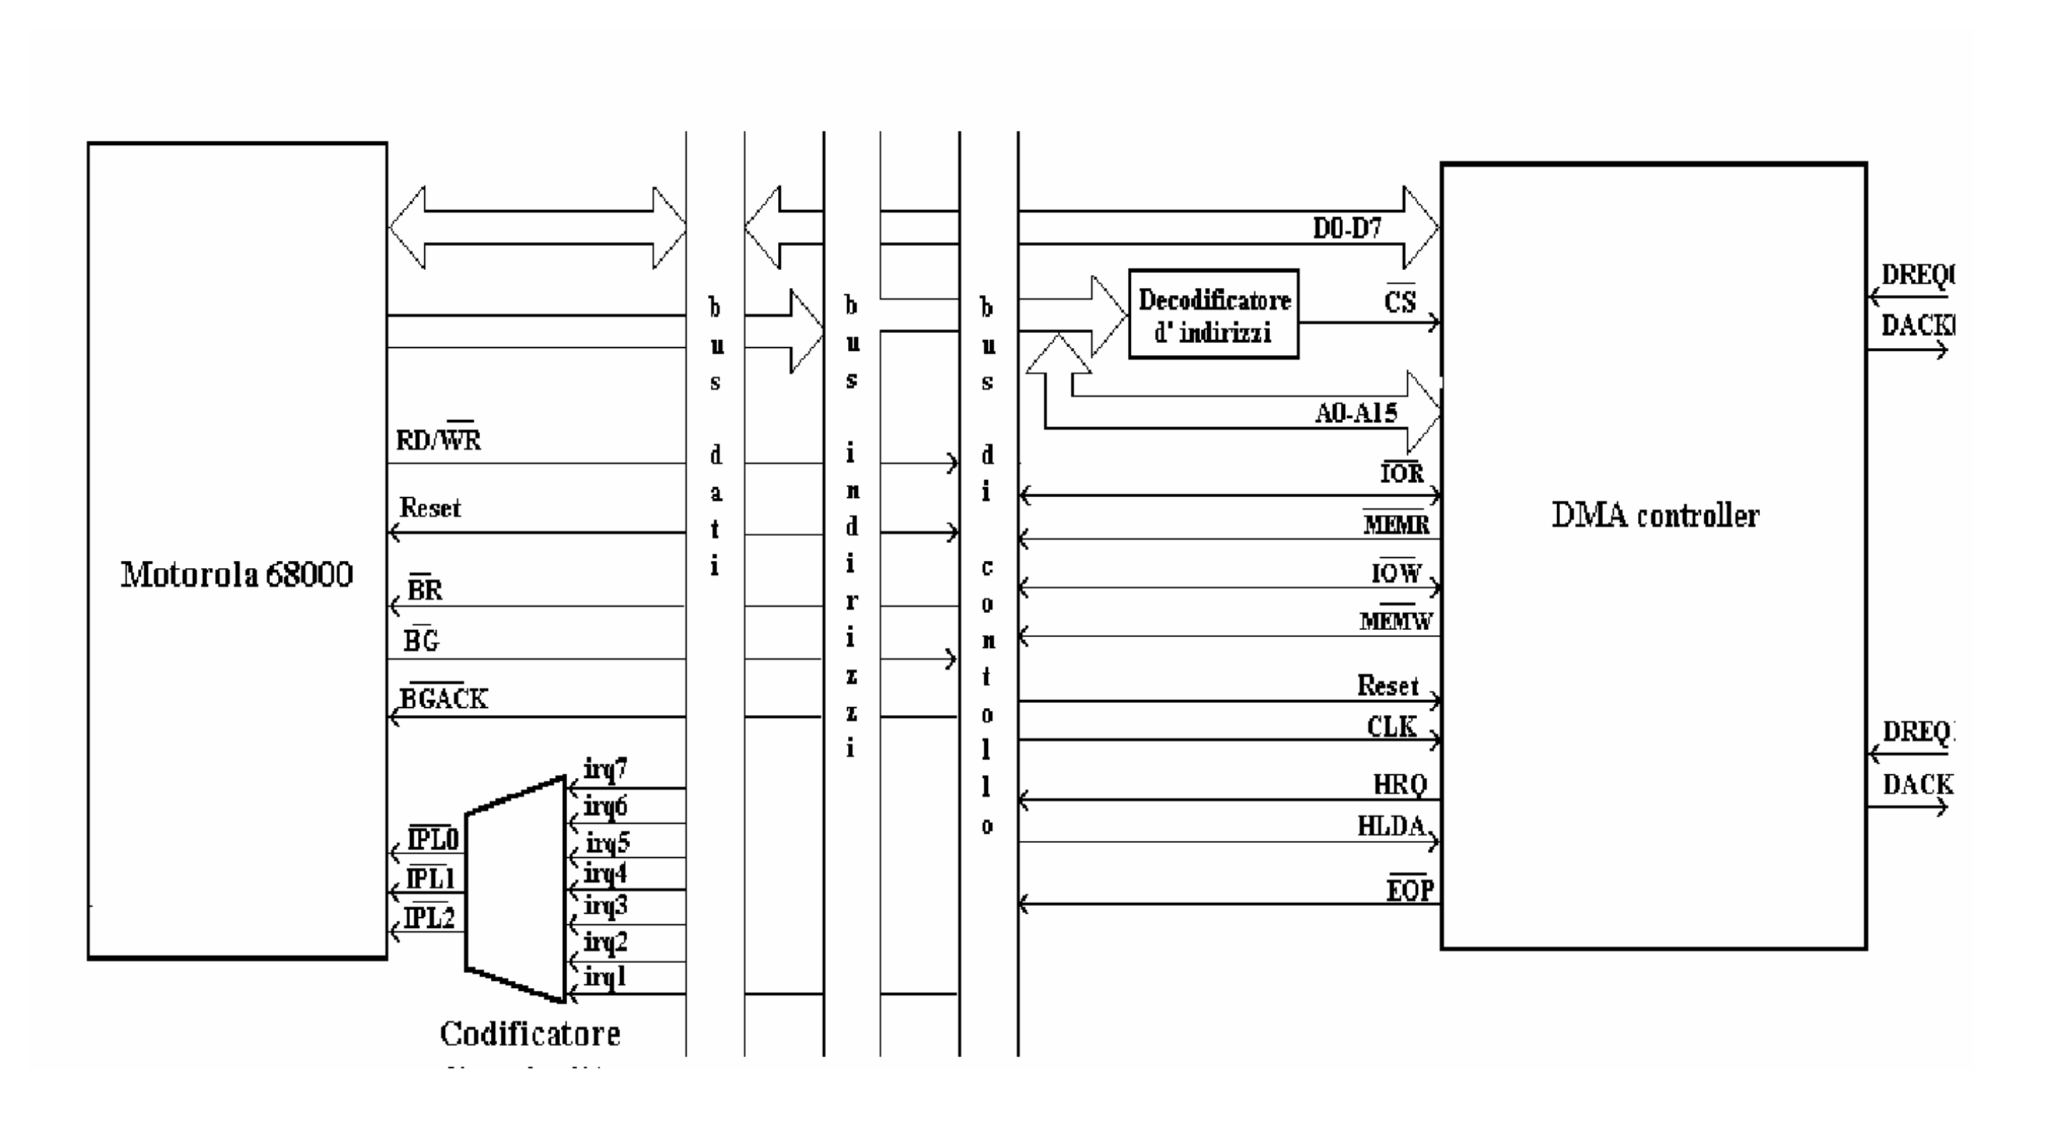
\includegraphics[width=.7\textwidth]{img/architettura-dma.png}
    \caption{Montaggio del componente DMA rispetto al sistema generale}
    \label{img:architettura-dma}
\end{figure}

Una volta compresa l'architettura del sistema, possiamo analizzare il significato dei bit dei vari registri interni.

\paragraph{Registro Mode}
Il registro Mode (uno per canale) è descritto nella Tabella~\ref{tab:MODE-8237}.
\begin{table}[ht]
    \centering
    \begin{tabular}{|c|p{11cm}|}
    \hline
    \textbf{Bit} & \textbf{Significato} \\ \hline
    0 & Instrada il dato su un canale: 0 per il canale 0, 1 per il canale 1 \\ \hline
    1-2 & Non utilizzati \\ \hline
    3 & Direzione di trasferimento: 0 = da memoria a interfaccia, 1 = da interfaccia a memoria \\ \hline
    4 & Abilita l'\textbf{Autoinizializzazione}: se impostato a 1, alla fine del conteggio resetta i registri con i valori di base \\ \hline
    5 & Incremento di CADDR (0) o decremento (1) \\ \hline
    6 & Non utilizzato \\ \hline
    7 & Modalità di trasferimento: 0 = Single, 1 = Block \\ \hline
    \end{tabular}
    \caption{Significato dei bit del registro MODE}
    \label{tab:MODE-8237}
\end{table}

\paragraph{Registro di Controllo}
Il registro di controllo del DMA controller è illustrato nella Tabella~\ref{tab:CTRL-8237}.
\begin{table}[ht]
    \centering
    \begin{tabular}{|c|p{11cm}|}
    \hline
    \textbf{Bit} & \textbf{Significato} \\ \hline
    0 & Termina conteggio per il canale 0 \\ \hline
    1 & Termina conteggio per il canale 1 \\ \hline
    2 & È stata inoltrata una richiesta al canale 0 \\ \hline
    3 & È stata inoltrata una richiesta al canale 1 \\ \hline
    4 & Non utilizzato \\ \hline
    5 & Abilita il trasferimento da memoria a memoria \\ \hline
    6 & Impone che in un trasferimento memoria-memoria l'indirizzo sorgente rimanga costante \\ \hline
    7 & Abilita il DMA controller \\ \hline
    \end{tabular}
    \caption{Significato dei bit del registro CTRL}
    \label{tab:CTRL-8237}
\end{table}

\newpage

\subsection{Implementazione in Motorola 68k}

Le implementazioni in ASIM con Motorola 68k sfruttano varie architetture definite nei file di configurazione. Una volta definita l'architettura, si stabilisce come gestire i registri e le periferiche (come il DMA). 

\subsubsection{Caso Memoria-Memoria}

Nel caso memoria-memoria, il DMA richiede una particolare definizione. Si devono definire:
\begin{itemize}
    \item l'area dati (origine e destinazione);
    \item gli intervalli per l'accesso ai registri interni del DMA.
\end{itemize}

\begin{lstlisting}
                ORG     $9500
origine         DC.B    0,1,2,3,4,5,6,7,8,9 * msg
destinazione    DS.B    34

* Definizione di indirizzo e offset per accesso ai registri DMA
dma             EQU     $2010
caddr0          EQU     0
caddr1          EQU     2
ccount1         EQU     3
cntrl           EQU     8
mode            EQU     11
reset           EQU     13
clearmf         EQU     14
writeamf        EQU     15
nbyte           EQU     34
\end{lstlisting}

Una volta definita la parte "statica", si passa alla parte operativa:

\begin{lstlisting}
    ORG         $8200 

    MOVE.W      #dma,A0           * Carico l'indirizzo del DMA

* Carico l'indirizzo di origine dei dati nel primo registro indirizzo
    MOVE.W      #origine,caddr0(A0)

* Carico l'indirizzo di destinazione nel secondo registro indirizzo
    MOVE.W      #destinazione,caddr1(A0)

* Numero di caratteri da trasferire
    MOVE.B      #nbyte,ccount1(A0)

* Configuro il primo canale: Block, incremento, autoinizializzazione
    MOVE.B      #$90,mode(A0)

* Configuro il secondo canale in modo analogo
    MOVE.B      #$91,mode(A0)

* Set del control register
    MOVE.B      #$A0,cntrl(A0)

* Ciclo caldo
LOOP    JMP     LOOP
\end{lstlisting}

Alla fine del trasferimento, occorre gestire l'interruzione scatenata. L'ISR ha come scopo il reset del DMA:

\begin{lstlisting}
        ORG     $8700

int7    MOVE.L  A0,-(A7)           * Salva il contesto
        MOVE.W  #dma,A0
        MOVE.B  #0,reset(A0)       * Resetta il DMA
        MOVE.L  (A7)+,A0           * Ripristina il registro
        RTE
\end{lstlisting}

\subsubsection{Caso Dispositivo $\rightarrow$ Memoria}
La configurazione che studiamo in questo paragrafo rappresenta due sistemi in comunicazione, uno in trasmissione e uno in ricezione tramite due PIA. La PIA in trasmissione manda continuamente caratteri alla PIA in ricezione, il DMA collegato al sistema in ricezione sposta i caratteri ricevuti dalla PIA verso la Memoria, senza passare per il processore. 
Presentiamo innanzitutto il sistema in trasmissione che denominiamo S1, che effettua il trasferimento con un semplice ciclo.

\begin{lstlisting}
***AREA DATI***
        ORG     $8000
MSG     DC.B    1,2,3,4,5,6
DIM     DC.B    6

***MAIN***
        ORG     $8200
PIADB   EQU     $2006
PIACB   EQU     $2007 


MAIN    JSR     DVBOUT 
        MOVEA.L #PIACB,A1 
        MOVEA.L #PIADB,A2 
        MOVEA.L #MSG,A0 
        MOVE.B  DIM,D0
        CLR     D1
        MOVE    D0,D2 
INVIO   MOVE.B  (A0)+,D1 
        MOVE.B  D1,(A2) 
        ADDQ    #-1,D2
        BNE     INVIO 

LOOP    JMP     LOOP 

DVBOUT  MOVE.B  #0,PIACB
        MOVE.B  #$FF,PIADB 
        MOVE.B  #%00100100
        RTS 
\end{lstlisting}

Osserviamo che in questo caso non effettuiamo l'handshaking, e non effettuiamo la lettura fittizia per assicurarci che CRB7 sia basso, semplciemente scriviamo sul PRB. Questo è dovuto al fatto che il DMA non possiede segnali per parlare direttamente con la PIA, quindi \textit{forziamo} una scrittura senza handshaking.
Procediamo con la presentazione del driver di un sistema che riceve un messaggio di 30 caratteri su una PIA e lo copia in memoria direttamente tramite un DMA. Assumiamo che la PIA sia collegata al canale 0 del DMA e che la linea di interruzione del DMA sia collegata sulla linea 7 del processore (Autovettore 31).

\begin{lstlisting}
***AREA DATI***
PIADA   EQU     $2004
PIACA   EQU     $2005

dma     EQU     $2010 
caddr0  EQU     0
ccount0 EQU     1
cntrl   EQU     8
request EQU     9
mode0   EQU     11
nbyte   EQU     30


        ORG     $8000
msg     DS.B    nbyte 

***AREA CODICE***
        ORG     $8200
MAIN    JSR     DVAIN 
        MOVE.W  SR,D0 
        ANDI.W  #$D8FF,D0 *stato utente, int abilitate 
        MOVE.W  D0,SR 

        MOVE.W  dma,A1 
        MOVE.B  #nbyte,ccount0(A1)
        MOVE.W  msg,caddr0(A1)
        MOVE    #$08,mode0(A1)
        MOVE    #$80,cntrl(A1)
        MOVE    #$08,request(A1)

LOOP    JUMP    LOOP 

DVAIN   MOVE    #0,PIACA
        MOVE.W  #00,PIADA 
        MOVE    #$00100101,PIACA 
        RTS 

**ISR FINE TRASFERIMENTO*** 
        ORG     $8700
        NOP 
        RTE 


\end{lstlisting}

\subsubsection{Caso Memoria $\rightarrow$ Dispositivo}
In questo caso, un dispositivo  deve trasmettere un messaggio da un'area di memoria verso una PIA usando il DMA. La PIA deve essere programmata per ricevere dati, quindi il porto va configurato in INPUT. Nell'esempio presentato a lezione, non si affronta la questione del trasferimento da PIA del sistema S1 a PIA del sistema S2, quindi il programma non funziona ed è presentato al solo scopo didattico di illustrare il passaggio da Memoria e Interfaccia dispositivo tramite DMA. 

\begin{lstlisting}
***AREA COSTANTI***
PIADA   EQU     $2004
PIACA   EQU     $2005

dma     EQU     $2010
caddr0  EQU     0
ccount0 EQU     1
cntrol  EQU     8
request EQU     9
mode0   EQU     11
nbyte   EQU     6

***AREA DATI*** 
        ORG     $8000
MSG     DC.B    1,2,3,4,5,6
DIM     DC.B    6

***AREA CODICE***
MAIN    JSR     PIAINIT
        MOVE.W  SR,D0 
        ANDI.W  #$D8FF,D0
        MOVE.W  D0,SR 

        MOVE.W  #dma,A1 
        MOVE.W  #nbyte,ccount0(A1)
        MOVE.W  #msg,caddr0(A1)
        MOVE    #$10000000,mode0(A1)
        MOVE    #$08,request(A1)

LOOP    JMP     LOOP 

PIAINIT MOVE    #0,PIACA 
        MOVE    #$00,PIADA 
        MOVE    #%00100100,PIACA 
        RTS 

\end{lstlisting}
\newpage 